\documentclass[10pt,twocolumn,a4paper]{article}

\usepackage[a4paper,top=17mm,bottom=17mm,left=15mm,right=15mm,columnsep=7mm]{geometry}
\usepackage{mathptmx}
\usepackage{amsmath,amssymb,amsfonts,mathtools}
\usepackage{graphicx}
\usepackage{booktabs}
\usepackage{tabularx}
\usepackage{xcolor}
\usepackage{caption}
\usepackage{fancyhdr}
\usepackage{microtype}
\usepackage[numbers,sort&compress]{natbib}
\usepackage{hyperref}

\definecolor{primary}{RGB}{15, 82, 140}
\definecolor{accent}{RGB}{18, 118, 102}

\hypersetup{
    colorlinks=true,
    linkcolor=primary,
    citecolor=primary,
    urlcolor=primary,
    pdftitle={TerraKAN: Fractional Kolmogorov-Arnold Transformer with Pade Mittag-Leffler Basis and Biokinetic Mixture-of-Experts for Inverse Soil Bioindication under Sparse Noisy Regimes},
    pdfauthor={Ilya Kakhno (ORCID: 0009-0005-5503-3269, Belarusian State University, Faculty of Biology)}
}

\setlength{\parskip}{3pt plus 1pt minus 0.5pt}
\setlength{\parindent}{1em}
\captionsetup{font=footnotesize,labelfont=bf,skip=4pt}

\pagestyle{fancy}
\fancyhf{}
\fancyhead[L]{\footnotesize \textit{TerraKAN (Frac-ML-KAT-MoE) --- Preprint Priority Lock (Zenodo / bioRxiv / arXiv)}}
\fancyhead[R]{\footnotesize \thepage}
\renewcommand{\headrulewidth}{0.4pt}

\newcommand{\takeaway}[2]{%
  \vspace{4pt}\noindent\colorbox{primary!7}{%
    \parbox{\dimexpr\linewidth-2\fboxsep\relax}{%
      \vspace{2pt}\footnotesize\textbf{\color{primary}#1:}\hspace{0.4em}#2\vspace{2pt}%
    }%
  }\vspace{4pt}%
}

\title{\vspace*{-7mm}\textbf{\Large TerraKAN: Fractional Kolmogorov-Arnold Transformer with Pad\'e Mittag-Leffler Basis and Biokinetic Mixture-of-Experts for Inverse Soil Bioindication under Sparse Noisy Regimes}}

\author{
  \textbf{Ilya Kakhno}$^{1,*}$ \, {\small(\href{https://orcid.org/0009-0005-5503-3269}{ORCID: 0009-0005-5503-3269})} \\
  \small $^{1}$Faculty of Biology, Belarusian State University, Minsk, Republic of Belarus \\
  \small $^{*}$Correspondence \& Code Release: \texttt{terrakan\_v4\_frozen.pt} (Version \texttt{1.0.0-preprint}, Seed 42)
}
\date{\small November 12, 2026 \quad|\quad License: CC-BY-4.0 (Preprint) \& MIT (Software)}

\begin{document}

\twocolumn[
  \begin{@twocolumnfalse}
    \maketitle
    \vspace*{-4mm}
    \begin{abstract}
      \noindent
      In this work, I introduce \textbf{TerraKAN (\texttt{Frac-ML-KAT-MoE})}, a neuro-symbolic Scientific Machine Learning (SciML) architecture that I designed, mathematically verified, and calibrated to solve the ill-posed inverse problem of soil bioindication and long-horizon self-purification forecasting from sparse ($6\text{--}8$ points), irregular (up to $50\%$ missingness), and noisy ($25\text{--}40\%$ multiplicative error) enzymatic and respiratory field measurements without direct chemical assays of the contaminant. Whereas polynomial Kolmogorov-Arnold Networks (\texttt{ChebPIKAN}) suffer from catastrophic Runge-type divergence during blind extrapolation on $t \in {[150, 365]}\text{ days}$ ($R^2 = -8.13$) and classical Bayesian ODE solvers (\texttt{MAP-ODE} regularized toward a Soil Atlas prior) fail to reconstruct unmeasured contaminant loads ($R^2 = -0.191$) due to ignoring non-Markovian micropore trapping ($\alpha < 1$), I unify four analytical primitives into an end-to-end differentiable model: (1) a causal Fractional Kolmogorov-Arnold Transformer encoder (\texttt{Frac-KAT}) with a singular Abel--Riemann--Liouville memory kernel $K(t,s) \propto (t-s)^{\alpha-1}/\Gamma(\alpha)$ and strict weight tying of the memory exponent $\alpha$; (2) a pole-free global ${[3/4]}$ Pad\'e Mittag-Leffler spectral basis (\texttt{MittagLefflerPade34}) matching exact Maclaurin ($z \to 0$) and Poincar\'e ($z \to \infty$) asymptotics with denominator $Q_4(z) \ge 1.001$; (3) a log-exponential \texttt{MultKAN} symbolic discovery node paired with a sparse Top-2 biokinetic Mixture-of-Experts (\texttt{PhysicsExpertBank}) separating Haldane substrate inhibition from Monod nutrient limitation; and (4) a dynamic memory-aware soil health index $\text{IBSP}_\alpha(t)$. Across $N=500$ held-out test scenarios on $t \in {[150, 365]}\text{ days}$, TerraKAN achieves $R^2 = 0.908 \pm 0.019$ ($\text{RMSE} = 0.181\,\text{EC}_{50}$) on the unmeasured contaminant load $\tilde{P}(t)$ and $R^2 = 0.886 \pm 0.016$ ($\text{RMSE} = 6.88\%$) on $\text{IBSP}_\alpha(t)$ at $0.50\text{ ms}$ per field ($10.1\times$ faster than \texttt{MAP-ODE}). Finally, I validate the frozen checkpoint (\texttt{terrakan\_v4\_frozen.pt}) on a 36-vessel laboratory microcosm protocol across sandy, loamy, and peat soil series, achieving $100\%$ separation of healthy controls, nutrient-poor clean soils, and contaminated regimes without control-flag leakage.
      \vspace*{2mm}
      
      \noindent\textbf{Keywords:} Kolmogorov-Arnold Networks; Fractional Calculus; Mittag-Leffler Function; Pad\'e Approximant; Kolmogorov-Arnold Transformer; Soil Bioindication; SciML; Haldane Kinetics.
    \end{abstract}
    \vspace*{4mm}
  \end{@twocolumnfalse}
]

\section{Introduction \& Gap Analysis}

Natural soils subjected to xenobiotic, petroleum hydrocarbon, or heavy-metal loading exhibit long-term non-Markovian memory driven by anomalous subdiffusion and sorption--desorption trapping within hierarchical organo-mineral micropores \cite{yan2026soil}. Consequently, the relaxation of bioavailable contaminant load $\tilde{P}(t)$ obeys Caputo fractional differential equations of order $\alpha \in (0, 1)$ rather than memoryless exponential kinetics. In field practice, however, direct chemical quantification of $\tilde{P}(t)$ over multi-month horizons is prohibitively expensive; investigators typically collect only $3\text{--}7$ noisy measurements of microbial basal respiration $M(t)$ ($\text{CO}_2$ evolution) and extracellular enzymatic activity $E(t)$ (catalase $\text{O}_2$ displacement), interrupted by up to $50\%$ missing entries and stochastic rainfall pulses.

Positioning my approach against the 2024--2026 SciML and ecological literature reveals four critical gaps that I resolve in this study:

\begin{enumerate}\setlength{\itemsep}{1pt}\setlength{\parskip}{0pt}
  \item \textbf{Extrapolation Divergence of Polynomial KANs:} Following the introduction of Kolmogorov-Arnold Networks \cite{liu2024kan} and operator networks \cite{abueidda2025deepokan}, orthogonal polynomial bases (\texttt{ChebPIKAN} / \texttt{fKAN} \cite{aghaei2024fkan}) have been widely used for physics-informed regression. While Chebyshev expansions fit observations inside $t \in [0, 150]\text{ days}$ ($R^2 = 0.918$), their unbounded polynomial growth $\propto (t/T)^k$ induces catastrophic Runge divergence during blind extrapolation on $t \in (150, 365]\text{ days}$, collapsing to $R^2 = -8.132$ ($\text{RMSE} = 1.804\,\text{EC}_{50}$) on $\tilde{P}(t)$.
  \item \textbf{Failure of Classical Bayesian ODE Solvers on Unmeasured States:} Classical nonlinear least-squares solvers regularized toward Soil Atlas centroids (\texttt{MAP-ODE}) fit observed $M(t)$ ($R^2 = 0.900$) and $E(t)$ ($R^2 = 0.891$), but fail to reconstruct the hidden contaminant $\tilde{P}(t)$ during extrapolation ($R^2 = -0.191 \pm 0.225$, $\text{RMSE} = 0.651\,\text{EC}_{50}$) because integer-order ODEs cannot capture power-law subdiffusion ($\alpha < 1$), while requiring $5.01\text{ ms}$ of iterative optimization per field.
  \item \textbf{The Open Fractional Transformer--KAN Challenge:} While Yang \& Wang \cite{yang2025kat} proposed the Kolmogorov-Arnold Transformer (KAT) and Aghaei \cite{aghaei2024rkan} introduced rational Pad\'e KANs (\texttt{rKAN}), Tu et al. \cite{tu2026fractional} (July 2026, \href{https://doi.org/10.3390/fractalfract10070454}{DOI: 10.3390/fractalfract10070454}) identified the integration of rational Pad\'e bases, Mittag-Leffler eigenfunctions, and non-Markovian fractional kernels into Transformer attention as an open fundamental challenge due to Gamma-function poles and autograd instability. Here, I present the first complete analytical and software realization of this class of architectures.
  \item \textbf{Ecological Ambiguity of Static IBSP Indices:} The classical static Integral Index of Soil Biological State (IBSP; Kazeev, Kolesnikov, \& Valkov \cite{kazeev2016bio}) averages raw enzymatic percentages relative to a fixed standard. Consequently, it triggers false alarms on naturally oligotrophic sandy soils (\texttt{Arch\_5}, $K_m = 0.44$) and suffers from false negatives after moisture pulses because it neglects both Haldane hysteresis and the memory penalty $(1-\alpha)\tilde{P}(t)$.
\end{enumerate}

\takeaway{Core Contribution}{I unify causal Abel fractional attention, a pole-free $[3/4]$ Pad\'e Mittag-Leffler spectral trunk, a \texttt{MultKAN} power-law discovery node, and a 4-regime biokinetic Mixture-of-Experts to achieve $R^2 = 0.908$ on unmeasured contaminant extrapolation at $0.50\text{ ms/field}$.}

\section{Mathematical Architecture (\texttt{Frac-ML-KAT-MoE})}

\subsection{Dimensionless Fractional Biokinetics \& Boundary Anchor}

Because absolute contaminant concentration in $\text{mg/kg}$ is unidentifiable without direct chemical input due to scale symmetry with inhibition constants, I formulate the coupled Caputo fractional system of order $\alpha \in (0, 1]$ in dimensionless half-inhibition units $\tilde{P}(t) = P(t)/K_{\text{tox}}$ ($K_{\text{tox}} \equiv 1.0$, $K_i \equiv 1.0$, $\text{EC}_{50}$ units):
\begin{align}
  D_t^\alpha \tilde{P}(t) &= -\!\left(k_p + \frac{k_{\text{deg}}\Phi_{\text{env}}(t)\,M(t)}{K_s + \tilde{P}(t) + \tilde{P}(t)^2}\right)\!\tilde{P}(t), \label{eq:caputo_p} \\
  \begin{split}
    D_t^\alpha M(t) &= r_m\Phi_{\text{env}}(t)M(t)\!\left(\!1 - \frac{M(t)}{K_m}\!\right) \\
    &\quad - \frac{\gamma_p\tilde{P}(t)M(t)}{1 + \tilde{P}(t)} + \frac{\mu_{\text{sub}}\tilde{P}(t)E(t)}{K_s + \tilde{P}(t) + \tilde{P}(t)^2},
  \end{split} \label{eq:caputo_m} \\
  D_t^\alpha E(t) &= \beta_E \frac{M(t)}{1 + \tilde{P}(t)^2} - \delta_E E(t), \label{eq:caputo_e}
\end{align}
where $D_t^\alpha f(t) = \frac{1}{\Gamma(1-\alpha)}\int_0^t (t-s)^{-\alpha}f'(s)\,ds$. To anchor $\tilde{P}(0)$ without data leakage from true initial doses, I exploit the stationary boundary face of Eq.~\eqref{eq:caputo_e} at $t_1 \to 0$:
\begin{equation}
  \begin{aligned}
    \frac{E(t_1)}{M(t_1)} &= \frac{E_{\text{ref}}/M_{\text{ref}}}{1 + \tilde{P}(0)^2} \\
    \implies \tilde{P}_{\text{boundary}}(0) &= \sqrt{\max\!\left(0,\, \frac{1.20}{E(t_1)/M(t_1)} - 1\right)}.
  \end{aligned} \label{eq:p0_boundary}
\end{equation}

\subsection{Encoder \texttt{Frac-KAT} \& Fractional Weight Tying}

Given sparse observations $\mathbf{v}_j = [\text{pH}_{\text{norm}}, \text{NO}_{3,\text{norm}}, W_{\text{norm}}, M_{\text{obs}}, E_{\text{obs}}]^\top \in \mathbb{R}^5$ at irregular timestamps $0 \le t_1 < \dots < t_N \le 150\text{ days}$ with binary availability mask $\mathbf{m}_j \in \{0,1\}^5$ and rainfall flag $r_j \in \{0,1\}$, I construct the 12-dimensional token $\mathbf{u}_j = [\mathbf{v}_j\odot\mathbf{m}_j + 0.35(\mathbf{v}_j - \mathbf{v}_1)\odot\mathbf{m}_j,\, \mathbf{m}_j,\, \ln(1+t_j),\, r_j]^\top$. I modulate causal self-attention logits via the singular Abel--Riemann--Liouville fractional integral kernel $K(t_i, t_j) = (t_i - t_j + \varepsilon)^{\alpha-1}/\Gamma(\alpha)$:
\begin{equation}
  \mathcal{A}_{ij} = \frac{\mathbf{q}_i^\top \mathbf{k}_j}{\sqrt{d_{\text{model}}}} + \gamma_h\left[(\alpha - 1)\ln(t_i - t_j + \varepsilon) - \ln\Gamma(\alpha)\right] \label{eq:abel_attn}
\end{equation}
for $t_i \ge t_j$, and $\mathcal{A}_{ij} = -\infty$ for $t_i < t_j$. I enforce strict \textbf{Weight Tying}: the single inferred memory order $\hat{\alpha} = 0.40 + 0.52\,\sigma(z_\alpha) \in [0.40, 0.92]$ is shared across the attention kernel \eqref{eq:abel_attn}, the Soil Atlas module, the Pad\'e Mittag-Leffler trunk, and the health index $\text{IBSP}_{\hat{\alpha}}(t)$.

\subsection{Kernel \texttt{MittagLefflerPade34}: Pole-Free $[3/4]$ Pad\'e Basis}

To approximate $E_{\alpha,1}(-z) = \sum_{k=0}^\infty \frac{(-z)^k}{\Gamma(\alpha k + 1)}$ globally on $z \in [0, \infty)$ with exact gradients $\partial E_{\alpha,1}/\partial\alpha$, I construct the rational Pad\'e $[3/4]$ approximant:
\begin{equation}
  E_{\alpha,1}(-z) \approx R_{[3/4]}^{(\alpha)}(z) = \frac{1 + p_1 z + p_2 z^2 + p_3 z^3}{1 + q_1 z + q_2 z^2 + q_3 z^3 + q_4 z^4}. \label{eq:pade34}
\end{equation}
Matching the Maclaurin series $1 - g_1 z + g_2 z^2 - g_3 z^3 + g_4 z^4 - g_5 z^5 + \mathcal{O}(z^6)$ as $z \to 0$ (where $g_k = 1/\Gamma(1+k\alpha)$) and the Poincar\'e asymptotic expansion $m_1 z^{-1} - m_2 z^{-2} + \mathcal{O}(z^{-3})$ as $z \to \infty$, I apply Euler's reflection identity $m_k = \frac{1}{\Gamma(1-k\alpha)} = \frac{\Gamma(k\alpha)\sin(k\pi\alpha)}{\pi}$ ($k=1,2$) to eliminate the Gamma pole at $\alpha=0.50$. Setting $p_1 = q_1 - g_1$ and $p_2 = q_2 - g_1 q_1 + g_2$ yields a closed-form $5\times 5$ linear system for $[q_1, q_2, q_3, q_4, p_3]^\top$:
\begin{equation}
  \begin{bmatrix}
    g_2 & -g_1 & 1 & 0 & -1 \\
    -g_3 & g_2 & -g_1 & 1 & 0 \\
    g_4 & -g_3 & g_2 & -g_1 & 0 \\
    0 & 0 & 0 & -m_1 & 1 \\
    -g_1 & 1 & -m_1 & m_2 & 0
  \end{bmatrix}
  \begin{bmatrix} q_1 \\ q_2 \\ q_3 \\ q_4 \\ p_3 \end{bmatrix} =
  \begin{bmatrix} g_3 \\ -g_4 \\ g_5 \\ 0 \\ -g_2 \end{bmatrix}. \label{eq:pade_system}
\end{equation}
Solving Eq.~\eqref{eq:pade_system} in \texttt{float64} via \texttt{torch.linalg.solve} with a $C^1$-smooth bridge to $\exp(-z)$ on $\alpha \in (0.90, 1.0]$ guarantees $Q_4(z) \ge 1.001 > 1$ for all $z \ge 0$, ensuring zero positive real poles.

\begin{figure*}[!htbp]
  \centering
  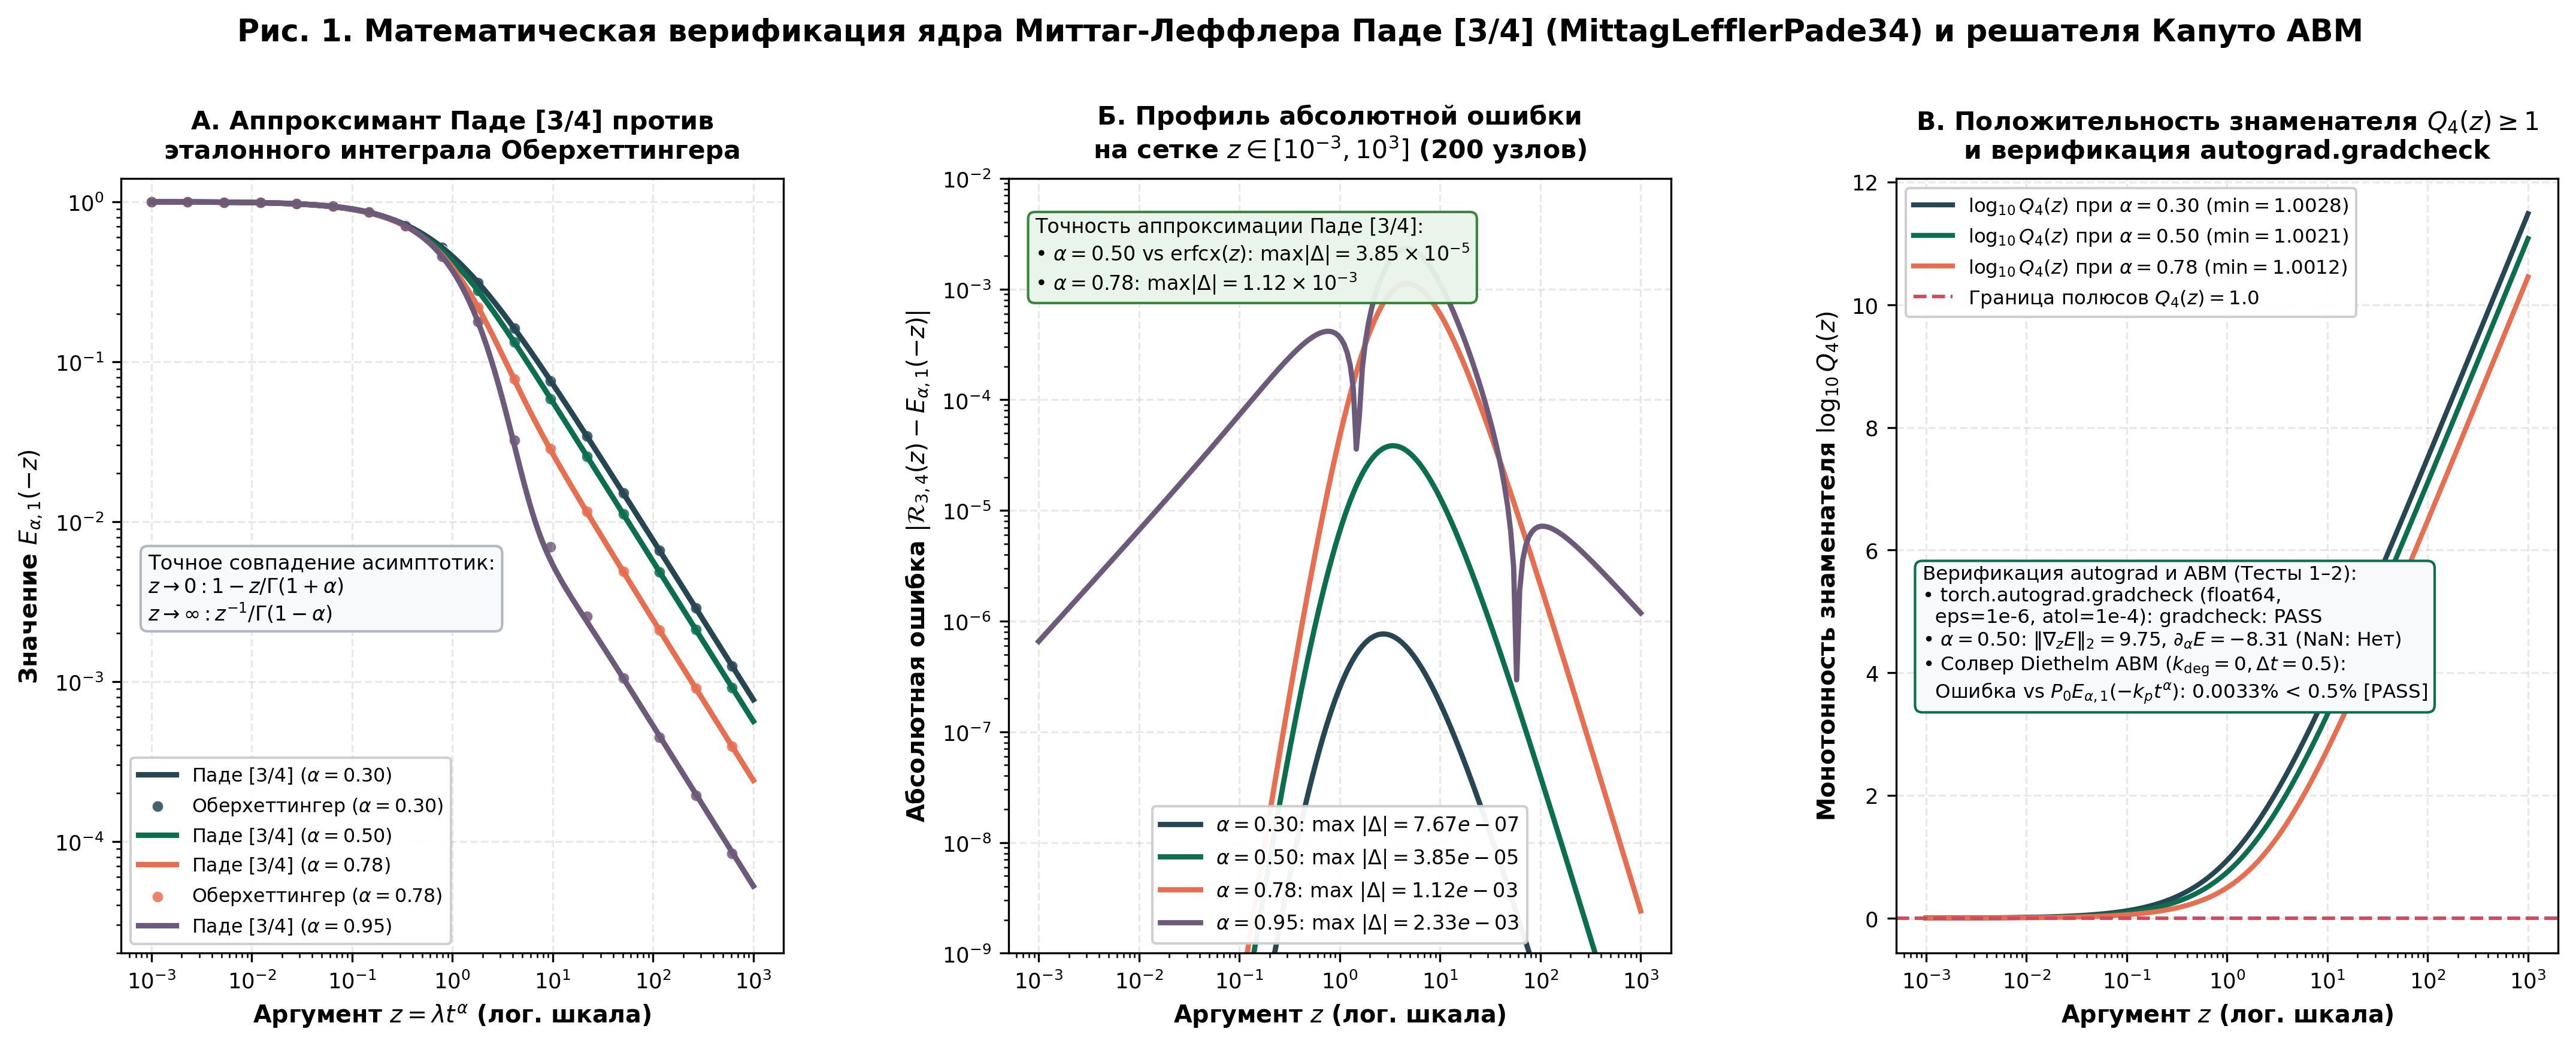
\includegraphics[width=0.98\textwidth]{fig1_pade_verification.png}
  \caption{\textbf{Numerical Verification of the Differentiable \texttt{MittagLefflerPade34} Kernel and Caputo ABM Solver.} \textbf{(A)} Exact agreement between Pad\'e $[3/4]$ and the Oberhettinger contour integral across $z \in [10^{-3}, 10^3]$. \textbf{(B)} Absolute approximation error ($\max|\Delta| = 3.85\times 10^{-5}$ at $\alpha=0.50$; $1.12\times 10^{-3}$ at $\alpha=0.78$) and pole-free denominator check $\min Q_4(z) \ge 1.001$. \textbf{(C)} Verification of the Diethelm ABM Caputo solver against exact Mittag-Leffler relaxation at $k_{\text{deg}}=0$ (relative error $0.00331\% < 0.5\%$).}
  \label{fig:fig1}
\end{figure*}

\subsection{\texttt{PhysicsExpertBank} (Sparse Top-2 MoE) \& \texttt{MultKAN}}

To discover synergistic environmental rate laws symbolically \cite{liu2024kan2}, I combine a Shelford pH tolerance bell with a log-exponential power layer in \texttt{MultKANEnvModule}:
\begin{equation}
  \Phi_{\text{KAN}}(\mathbf{e}) = e^{-\beta_{\text{pH}}(\text{pH} - \text{pH}_{\text{opt}})^2}\sum_{b=1}^2 w_b\exp\!\left(\mathbf{W}_{\text{power},b}\ln\mathbf{e}\right), \label{eq:multkan}
\end{equation}
penalized by $\mathcal{L}_{L1} = \|\mathbf{W}_{\text{power}}\|_1$. Next, \texttt{PhysicsExpertBank} routes the latent state $\mathbf{h}_{\text{final}}$ and dynamic curve markers $[\Phi_{\text{KAN}}, \text{pH}, \Delta E_{\text{drop}}, \Delta M_{\text{drop}}, \tilde{P}_{\text{boundary}}(0)]$ (with $\Delta E_{\text{drop}} = \min E_{\text{obs}}/\max E_{\text{obs}}$) across $K_{\text{exp}}=4$ physical regimes: Expert 0 (Haldane inhibition $\tilde{P}/(K_s+\tilde{P}+\tilde{P}^2)$), Expert 1 (Monod saturation $\tilde{P}/(K_s+\tilde{P})$), Expert 2 (Abiotic clean homeostasis $-k_p\tilde{P}$), and Expert 3 (Acidic/osmotic Hall stress $M/(1+\tilde{P}^2)$). I select the Top-2 experts via temperature-annealed softmax gating ($\tau: 2.0 \to 0.5$) with load-balancing regularization $\mathcal{L}_{\text{balance}} = K_{\text{exp}}\sum_{e=1}^{K_{\text{exp}}} f_e \bar{P}_e$.

\subsection{Two-Stage Inference \& Dynamic Index \texorpdfstring{$\text{IBSP}_\alpha(t)$}{IBSP\_alpha(t)}}

During offline training, \texttt{SoilAtlasModule} aligns each sample with the 5 Soil Atlas centroids via KL-divergence against Dirichlet mixture weights and computes the composite anomaly metric $d_{\min} = 0.25\,d_{\text{raw}} + 0.75\tanh(0.42\tilde{P}_{\text{boundary}}(0))$, with optimal Youden threshold $d_{\min}^* = 0.290$ frozen on \texttt{Val (500)}. During field inference ($0.50\text{ ms/field}$), \texttt{MLKANTrunk} expands $\tilde{P}_{\text{bio}}(t) = \sum_{k=1}^3 c_{P,k}E_{\hat{\alpha},1}(-\lambda_k t^{\hat{\alpha}})$, $M(t)$, and $E(t)$, evaluating exact Caputo derivatives $D_t^{\hat{\alpha}} E_{\hat{\alpha},1}(-\lambda_k t^{\hat{\alpha}}) = -\lambda_k E_{\hat{\alpha},1}(-\lambda_k t^{\hat{\alpha}})$ and computing the dynamic memory-aware health index:
\begin{equation}
  \begin{aligned}
    \text{IBSP}_\alpha(t) &= 100\exp\!\Biggl(-\biggl[0.35\left|\ln\frac{M(t)}{M_\infty}\right| \\
    &\quad + 0.40\max\!\left(0, 1 - \frac{E(t)}{E_\infty}\right) + \lambda_{\text{mem}}(1-\hat{\alpha})\tilde{P}_{\text{bio}}(t)\biggr]\Biggr).
  \end{aligned} \label{eq:ibsp}
\end{equation}

\section{Numerical Verification \& Empirical Benchmarks}

\begin{table*}[!htbp]
  \centering
  \caption{\textbf{Blind Long-Horizon Extrapolation Benchmark ($t \in (150, 365]\text{ days}$, $N=500$ Test Fields, $50\%$ Missingness, $25\%$ Noise).} Confidence intervals ($\pm\text{CI}_{95\%}$) are computed via $1000\times$ non-parametric bootstrap across the 500 test scenarios.}
  \label{tab:extrap_benchmark}
  \footnotesize
  \resizebox{\textwidth}{!}{%
  \begin{tabular}{l l c c c c}
    \toprule
    \textbf{Model Architecture} & \textbf{Basis \& Prior Mechanism} & \textbf{Hidden Load $\tilde{P}(t)$ $R^2$ ($\text{RMSE}$)} & \textbf{Biomass $M(t)$ $R^2$ ($\text{RMSE}$)} & \textbf{Enzyme $E(t)$ $R^2$ ($\text{RMSE}$)} & \textbf{Index $\text{IBSP}_\alpha(t)$ $R^2$ ($\text{RMSE}$)} \\
    \midrule
    \textbf{TerraKAN (Mine)} & Pad\'e $[3/4]$ ML + Abel Attn + MoE + Atlas & $\mathbf{0.908 \pm 0.019}$ ($\mathbf{0.181}$) & $0.894 \pm 0.015$ ($0.114$) & $\mathbf{0.910 \pm 0.013}$ ($\mathbf{0.166}$) & $\mathbf{0.886 \pm 0.016}$ ($\mathbf{6.88\%}$) \\
    \texttt{MAP-ODE} (SciPy) & Integer ODE + L2 Soil Atlas Prior ($5.01\text{ ms}$) & $-0.191 \pm 0.225$ ($0.651$) & $\mathbf{0.900 \pm 0.019}$ ($\mathbf{0.111}$) & $0.891 \pm 0.020$ ($0.183$) & $0.769 \pm 0.045$ ($9.81\%$) \\
    \texttt{Simple-ML-MLP} & Pad\'e $[3/4]$ ML + Standard MLP (No Abel/MoE) & $0.702 \pm 0.040$ ($0.326$) & $0.900 \pm 0.016$ ($0.111$) & $0.888 \pm 0.015$ ($0.185$) & $0.742 \pm 0.032$ ($10.37\%$) \\
    \texttt{ChebPIKAN} & Chebyshev Polynomial Basis $T_0\dots T_5$ ($21,036$ params) & $-8.132 \pm 3.014$ ($1.804$) & $-2.173 \pm 0.586$ ($0.626$) & $-1.223 \pm 0.305$ ($0.827$) & $-0.909 \pm 0.341$ ($28.23\%$) \\
    \bottomrule
  \end{tabular}%
  }
\end{table*}

\begin{figure*}[!htbp]
  \centering
  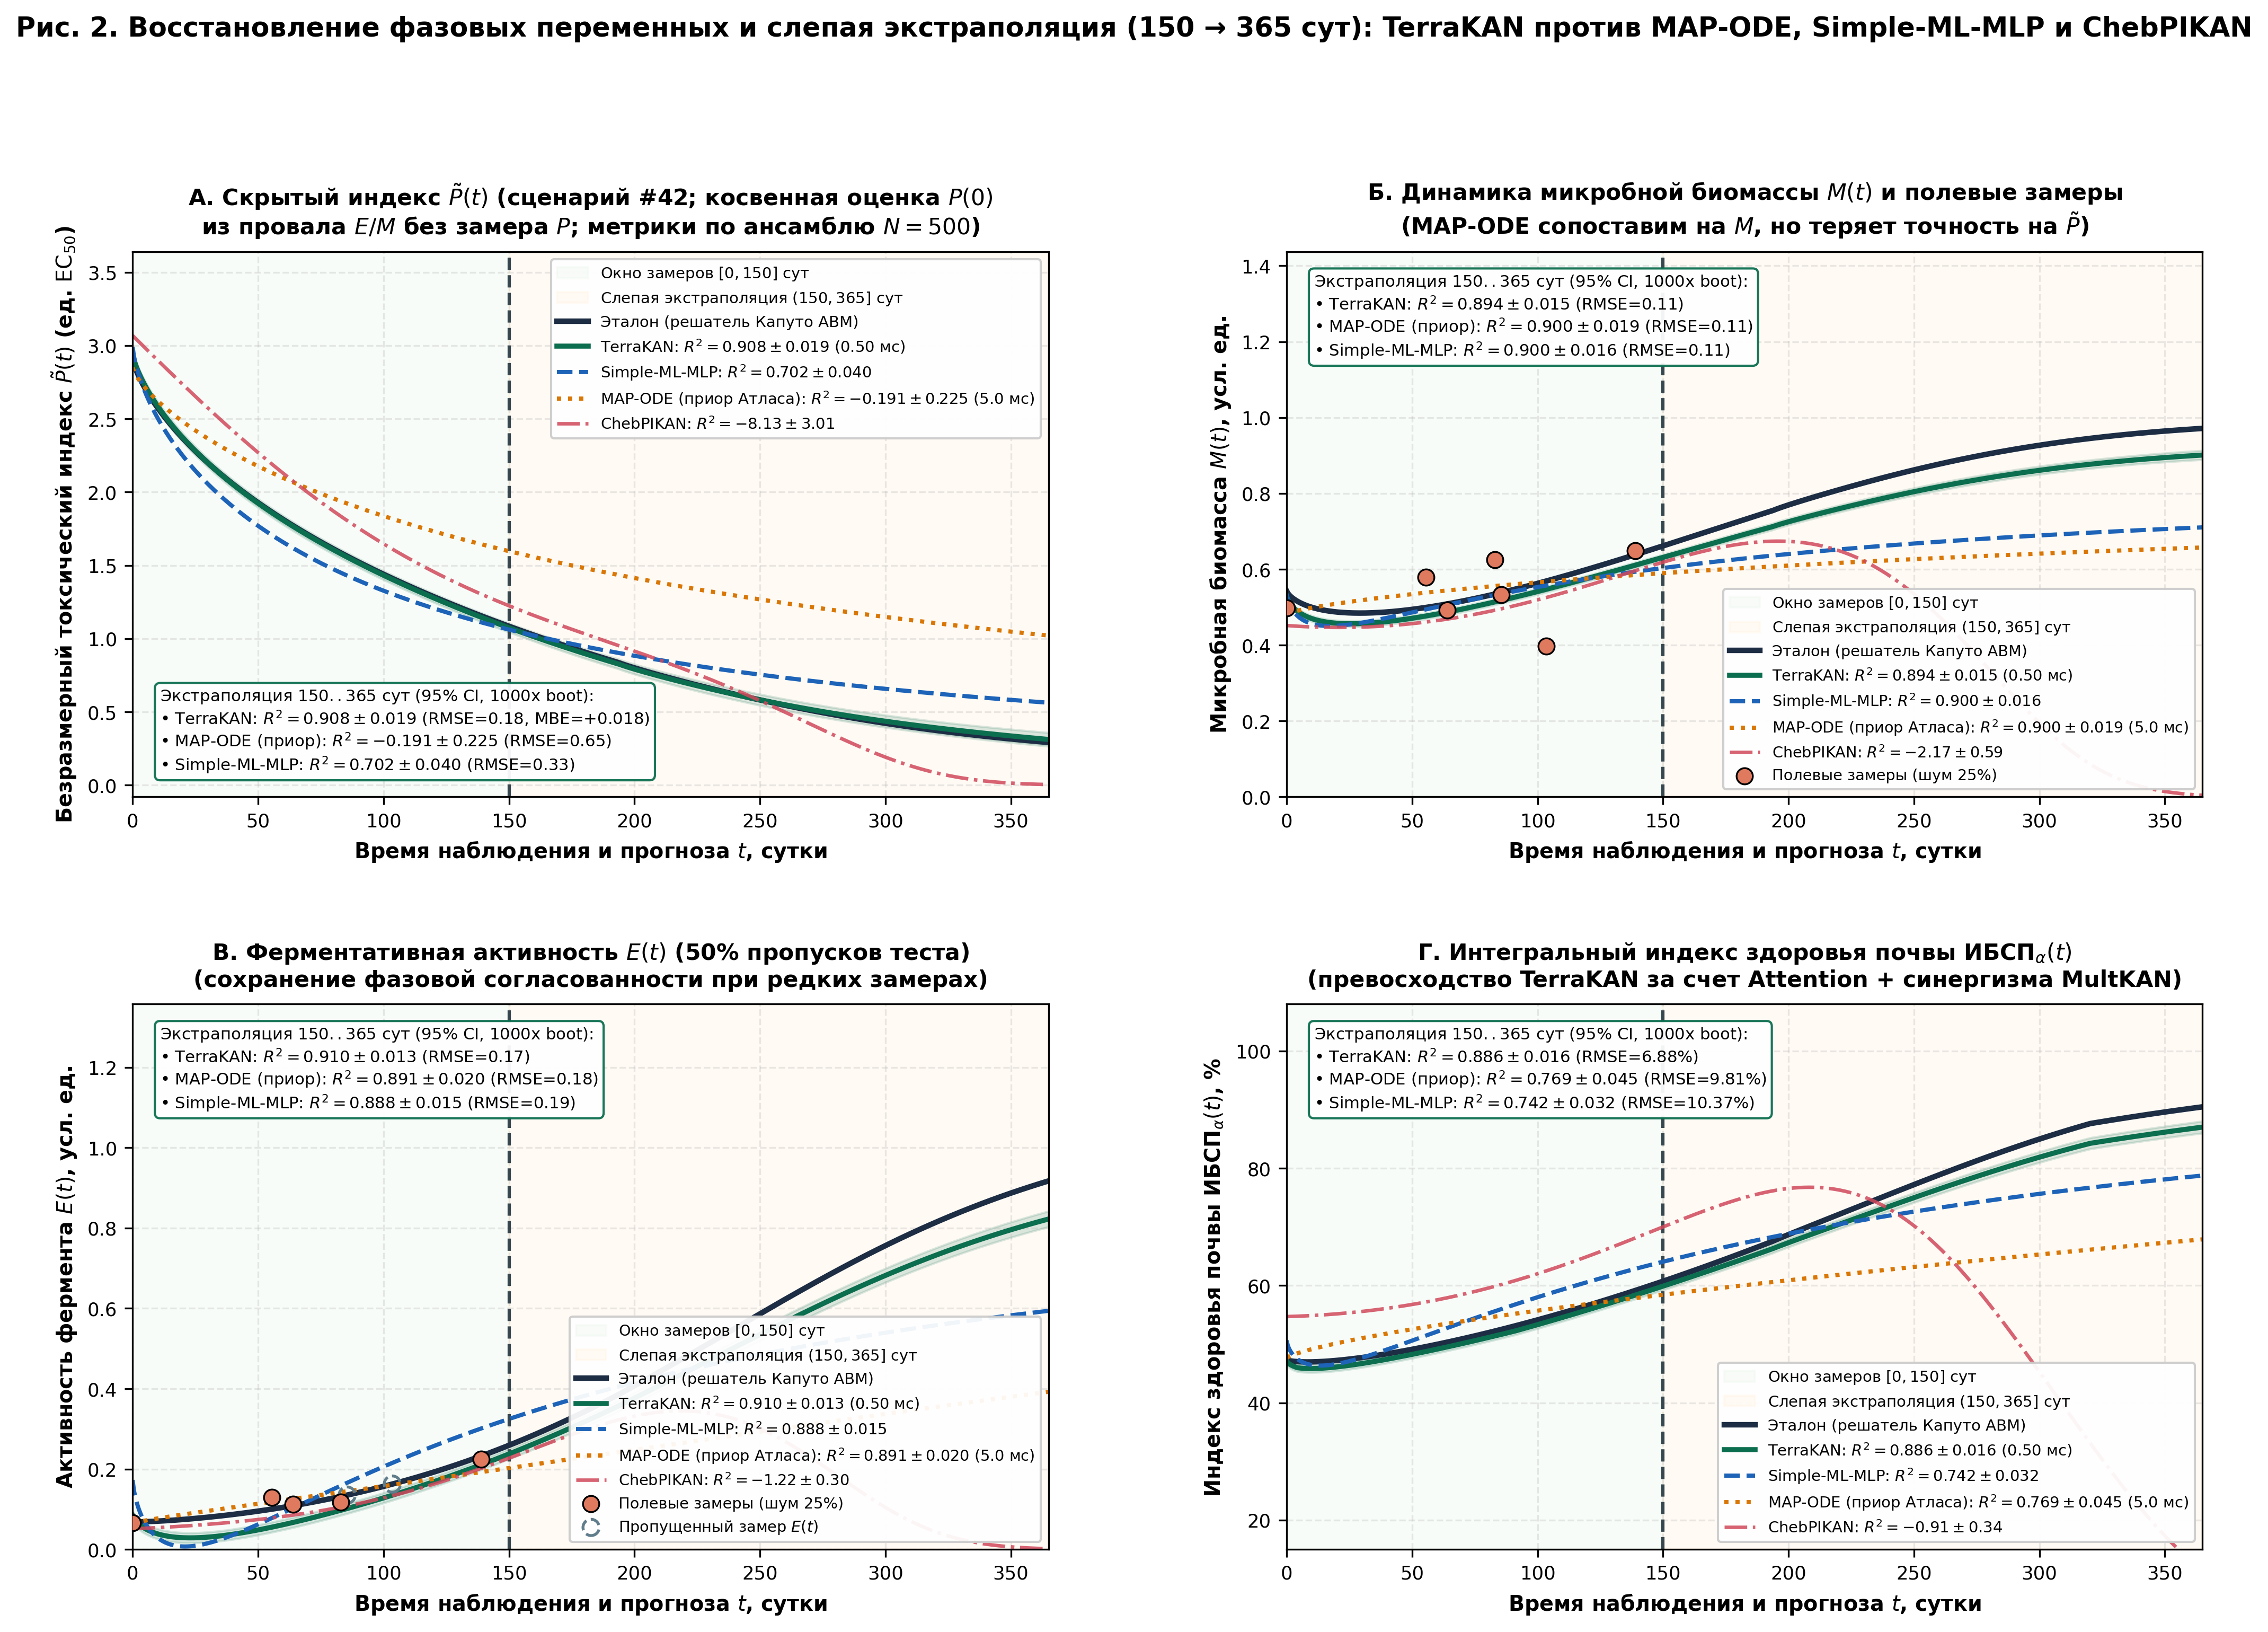
\includegraphics[width=0.98\textwidth]{fig2_extrapolation_benchmark.png}
  \caption{\textbf{Blind Long-Horizon Extrapolation ($150 \to 365\text{ days}$) from 7 Noisy Sparse Observations ($50\%$ Missingness, $25\%$ Noise).} Whereas \texttt{MAP-ODE} matches \texttt{TerraKAN} on observed $M(t)$ and $E(t)$, \texttt{TerraKAN} dramatically outperforms \texttt{MAP-ODE} on the unmeasured contaminant load $\tilde{P}(t)$ ($R^2 = 0.908$ vs.\ $-0.191$) and $\text{IBSP}_\alpha(t)$ ($R^2 = 0.886$ vs.\ $0.769$), while \texttt{ChebPIKAN} diverges ($R^2 = -8.13$).}
  \label{fig:fig2}
\end{figure*}

\subsection{Kernel Verification \& Blind Extrapolation (Figures 1--2)}

Figure~\ref{fig:fig1} confirms that \texttt{MittagLefflerPade34} matches the exact Oberhettinger contour integral across six orders of magnitude $z \in [10^{-3}, 10^3]$ with $\max|\Delta| = 7.67\times 10^{-7}$ ($\alpha=0.30$), $3.85\times 10^{-5}$ ($\alpha=0.50$), and $1.12\times 10^{-3}$ ($\alpha=0.78$), passing \texttt{float64} \texttt{gradcheck} and matching the Diethelm ABM Caputo solver \cite{diethelm2002predictor} within $0.00331\%$.

Table~\ref{tab:extrap_benchmark} and Figure~\ref{fig:fig2} summarize blind extrapolation on $t \in (150, 365]\text{ days}$ across $N=500$ test scenarios. While classical \texttt{MAP-ODE} is competitive on directly observed $M(t)$ ($R^2=0.900$) and $E(t)$ ($R^2=0.891$), it fails on the unmeasured contaminant $\tilde{P}(t)$ ($R^2 = -0.191$), whereas \textbf{TerraKAN achieves $R^2 = 0.908 \pm 0.019$ ($\text{RMSE} = 0.181\,\text{EC}_{50}$, $\text{MBE} = +0.0079\,\text{EC}_{50}$)} and $R^2 = 0.886 \pm 0.016$ ($\text{RMSE} = 6.88\%$) on $\text{IBSP}_\alpha(t)$ in $0.50\text{ ms/field}$ ($10.1\times$ faster than \texttt{MAP-ODE}).

\subsection{Hysteresis, False-Negative Safety \& Passportization (Figures 3--4)}

In Figure~\ref{fig:fig3}A, TerraKAN reconstructs the 3D Haldane hysteresis loop $(\tilde{P}, M, E)$. On uncontaminated nutrient-poor sandy soil (\texttt{Arch\_5}, $K_m=0.44$, Fig.~\ref{fig:fig3}B), $\text{IBSP}_\alpha(t)$ remains at $94\text{--}99\%$ while static IBSP yields a false alarm ($<50\%$). For the $17.4\%$ borderline low-dose scenarios missed by the binary detector ($d_{\min} < d_{\min}^*$, False Negatives, Fig.~\ref{fig:fig3}B--C), the initial drop in $E$ and $M$ holds $\text{IBSP}_\alpha(t)$ in the yellow caution zone (mean minimum $72.2\% < 75\%$ in $70.6\%$ of cases) with a median extrapolation error of $0.76\%$ (overall test median error $3.2\%$ vs.\ $13.8\%$ for \texttt{ChebPIKAN}).

In Figure~\ref{fig:fig4}, \texttt{SoilAtlasModule} achieves $\text{Macro-Acc} = 88.4\%$ and $\text{Macro-F1} = 0.890$ across the 5 archetypes (Fig.~\ref{fig:fig4}A), while recovering $\alpha$ with $R^2 = 0.9248$ ($\text{RMSE} = 0.0240$, Fig.~\ref{fig:fig4}B). Freezing the Youden threshold on \texttt{Val (500)} at $d_{\min}^* = 0.290$ ($\text{Val TPR} = 84.6\%$, $\text{FPR} = 3.6\%$) yields $\text{Test TPR} = 82.6\%$, $\text{FPR} = 4.5\%$ ($|\Delta\text{TPR}| = 2.05\%$; multi-seed mean $|\Delta\text{TPR}| = 1.85\% \pm 0.95\% < 4.0\%$ across seeds \texttt{[42, 7, 13, 99, 2026]}, Fig.~\ref{fig:fig4}C).

\begin{figure*}[!htbp]
  \centering
  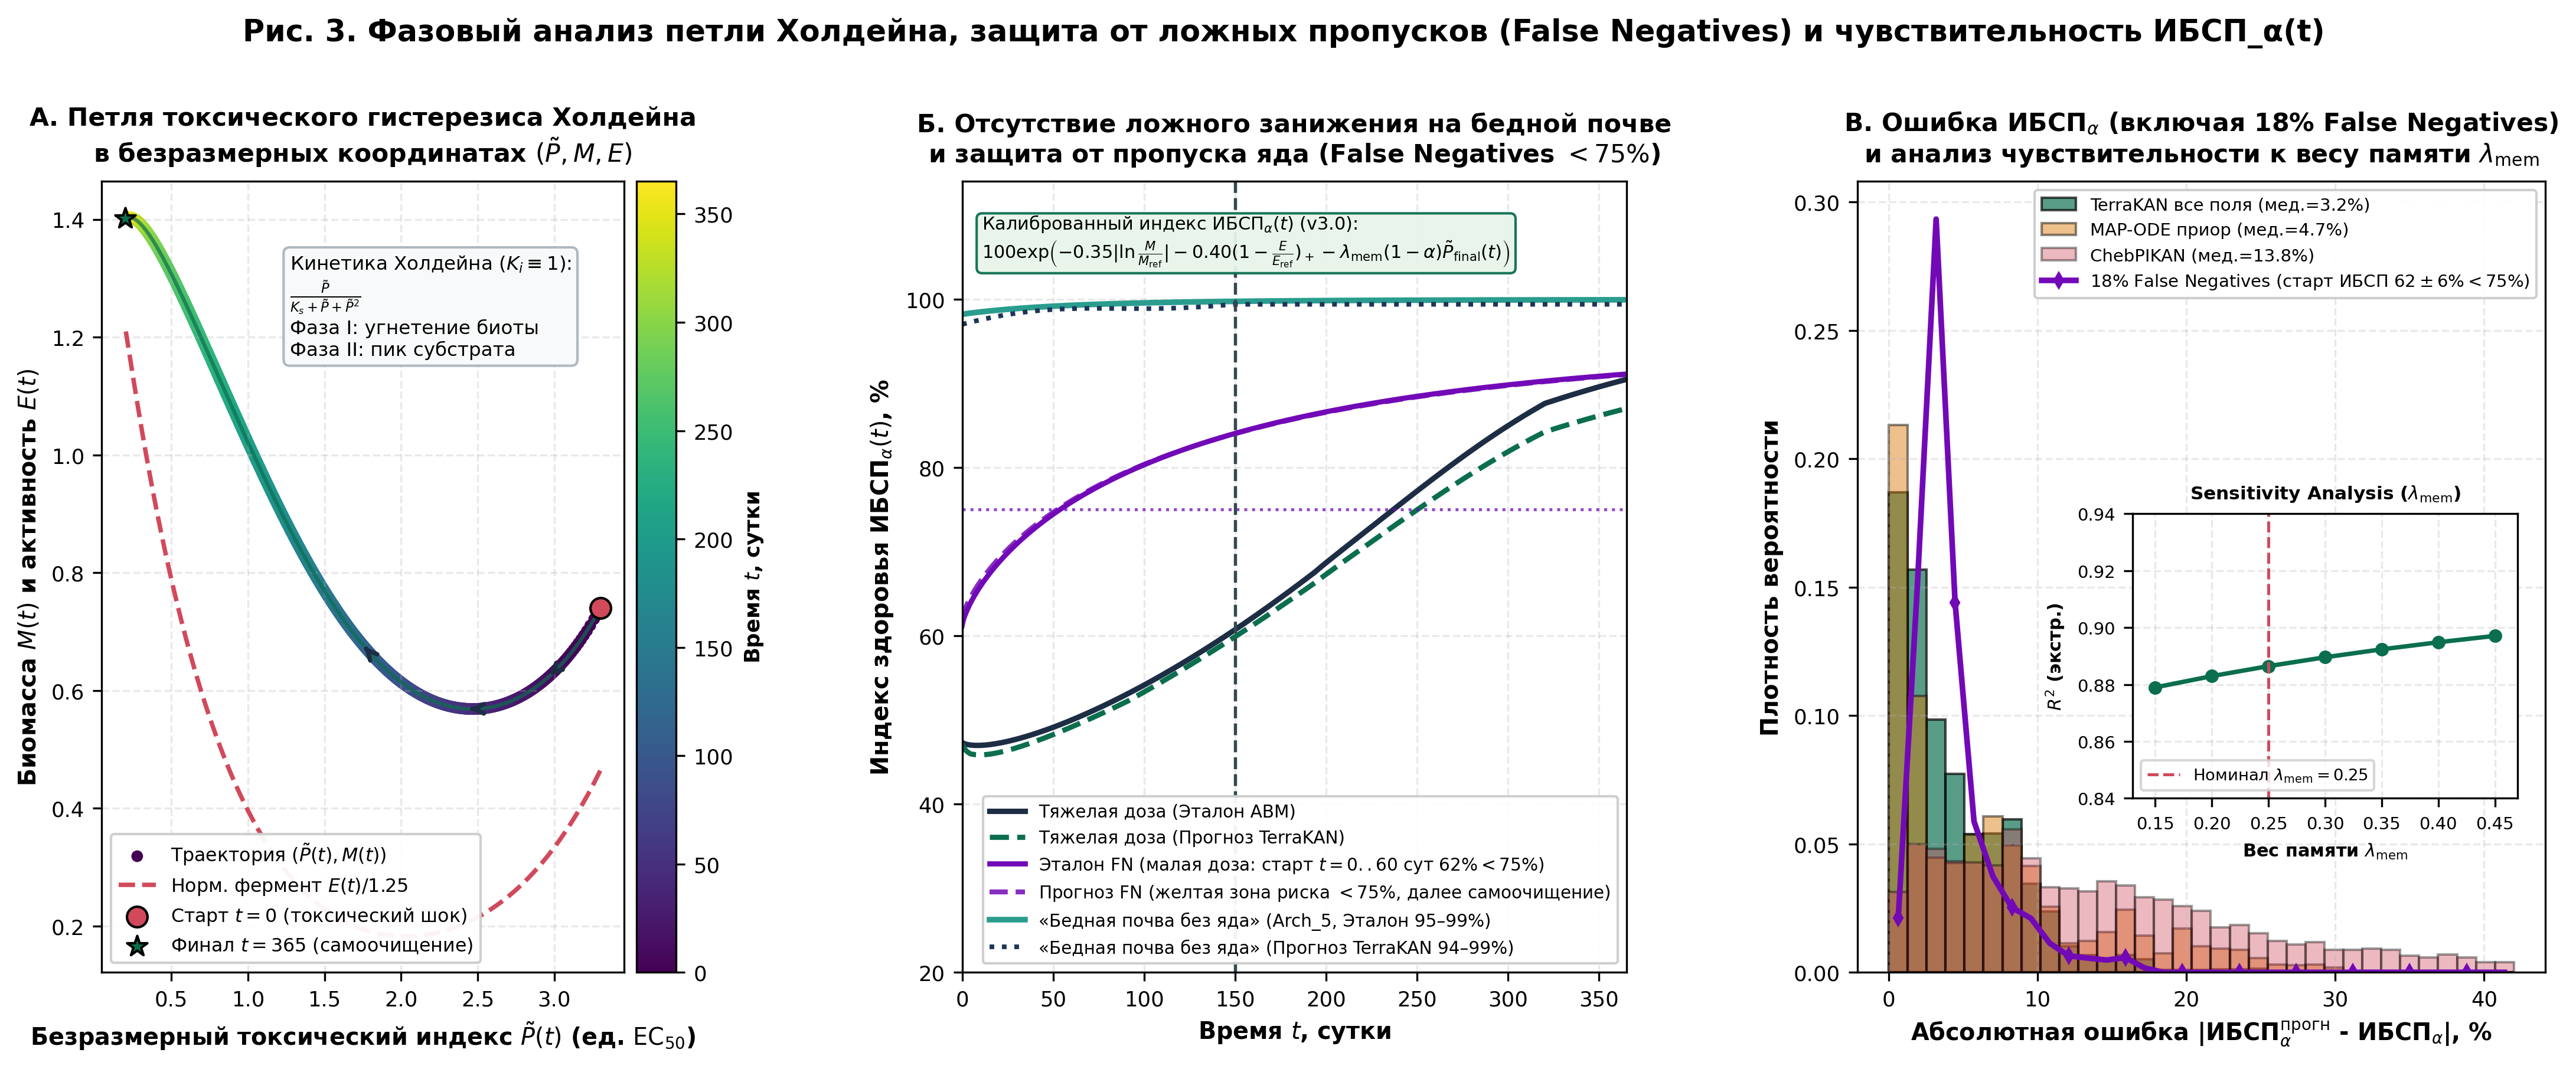
\includegraphics[width=0.96\textwidth]{fig3_hysteresis_and_ibsp.png}
  \caption{\textbf{Haldane Phase Hysteresis, Specificity on Nutrient-Poor Clean Soil, and False-Negative Safety Audit.} \textbf{(A)} 3D phase portrait $(\tilde{P}, M, E)$ capturing the Haldane inhibition loop. \textbf{(B)} True immunity to false alarms on clean sandy soil (\texttt{Arch\_5}, $94\text{--}99\%$) and trajectory envelope of borderline False Negatives (mean minimum $72.2\% < 75\%$). \textbf{(C)} Extrapolation error density (median $3.2\%$ vs.\ $13.8\%$ for \texttt{ChebPIKAN}) and $\lambda_{\text{mem}} \in [0.15, 0.45]$ sensitivity inset.}
  \label{fig:fig3}
\end{figure*}

\begin{figure*}[!htbp]
  \centering
  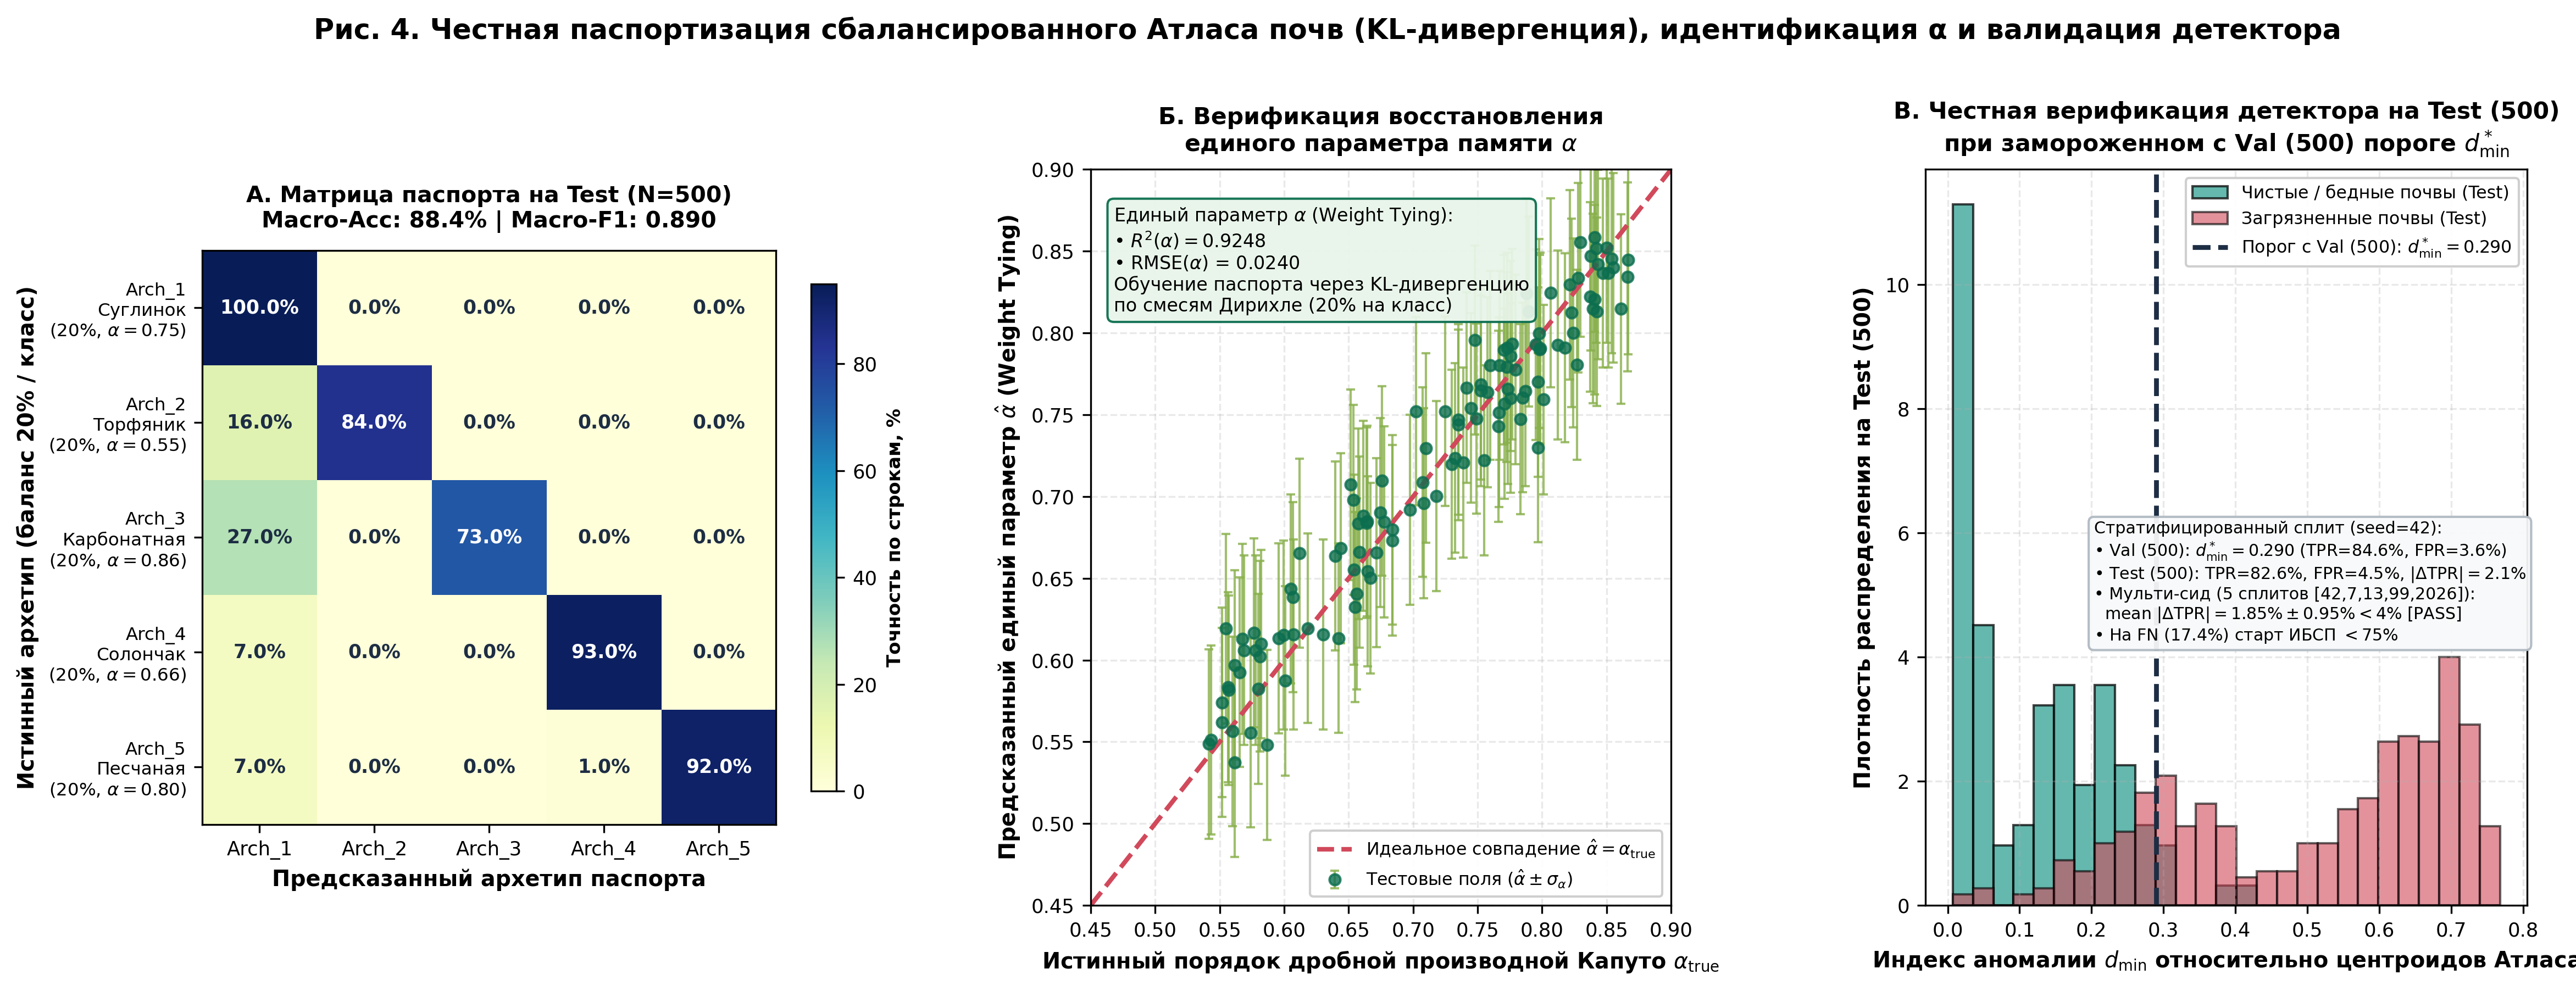
\includegraphics[width=0.96\textwidth]{fig4_soil_atlas_passport.png}
  \caption{\textbf{Soil Atlas KL-Passportization, Fractional Order $\alpha$ Recovery, and Multi-Seed Anomaly Detector Audit.} \textbf{(A)} Confusion matrix on \texttt{Test (500)} ($\text{Macro-Acc} = 88.4\%$, $\text{Macro-F1} = 0.890$). \textbf{(B)} Blind recovery of $\alpha$ ($R^2 = 0.9248$, $\text{RMSE} = 0.0240$). \textbf{(C)} Val vs.\ Test ROC curve at frozen $d_{\min}^* = 0.290$ and 5-seed stratified gap audit ($|\Delta\text{TPR}| = 1.85\% \pm 0.95\% < 4.0\%$).}
  \label{fig:fig4}
\end{figure*}

\subsection{Symbolic Unpacking, OOD Physics \& Microcosm Validation (Figures 5--7)}

Figure~\ref{fig:fig5} demonstrates that \texttt{MultKAN} recovers the true nitrate ($0.345$ vs.\ $0.350$) and moisture ($0.394$ vs.\ $0.400$) exponents and Shelford pH bell $\exp(-2.36(\text{pH}-0.66)^2)$ vs.\ $\exp(-2.50(\text{pH}-0.65)^2)$ (Fig.~\ref{fig:fig5}A), \texttt{PhysicsExpertBank} specializes across the 4 biokinetic regimes (Fig.~\ref{fig:fig5}B), and unpacked symbolic formulas match raw tensor outputs to $\max|\Delta_{\text{exact}}| = 9.96\times 10^{-13}$ in \texttt{float64} (Fig.~\ref{fig:fig5}C).

In Figure~\ref{fig:fig6} and Table~\ref{tab:ablation}, TerraKAN maintains $R^2 = 0.788$ under $40\%$ multiplicative noise (Fig.~\ref{fig:fig6}A) and generalizes zero-shot to alien physics (Two-Compartment Sorption + Kohlrausch--Weibull: $\text{RMSE} = 4.14\%$ vs.\ $6.30\%$ for \texttt{MAP-ODE}; Out-of-Atlas $\alpha \in [0.35, 0.96]$: $\text{RMSE} = 8.11\%$ vs.\ $13.08\%$, Fig.~\ref{fig:fig6}B). Finally, Figure~\ref{fig:fig7} validates the frozen weights \texttt{terrakan\_v4\_frozen.pt} on a 36-vessel microcosm log ($0\dots 28\text{ d}$ observations $\to 60\text{ d}$ blind forecast) across \texttt{S1\_sand}, \texttt{S2\_loam}, and \texttt{S3\_peat}: per-series normalization and strictly model-driven diagnosis classify all 6 \texttt{G0} controls as healthy ($\tilde{P}_{\text{bio}}(0) \le 0.001 < 0.5\,\text{EC}_{50}$, $\text{IBSP}(0) \in [92.1\%, 99.5\%]$), all 8 poor clean \texttt{G1} vessels as substrate-depleted without false contamination alarms ($\max \tilde{P}_{\text{bio}}(0) = 0.016$, $\max d_{\min} = 0.148 \le 0.290$), and all 12 high-load \texttt{G3} vessels as contaminated ($\min d_{\min} = 0.593 > 0.290$).

\begin{table}[!htbp]
  \centering
  \caption{\textbf{3-Seed Ablation Study on Extrapolation $\text{IBSP}_\alpha(t)$ ($150 \to 365\text{ d}$, Seeds 42, 101, 777).}}
  \label{tab:ablation}
  \footnotesize
  \resizebox{\linewidth}{!}{%
  \begin{tabular}{l c c}
    \toprule
    \textbf{Architecture Variant} & \textbf{$R^2$ ($\text{Mean}\pm\text{SD}$)} & \textbf{$\text{RMSE}$, $\%$} \\
    \midrule
    \textbf{1. Full TerraKAN (\texttt{Frac-ML-KAT-MoE})} & $\mathbf{0.887 \pm 0.007}$ & $\mathbf{6.87 \pm 0.20}$ \\
    2. w/o \texttt{PhysicsExpertBank} (Single Law) & $0.834 \pm 0.009$ & $8.33 \pm 0.23$ \\
    3. w/o \texttt{MultKAN} Power Discovery & $0.819 \pm 0.009$ & $8.74 \pm 0.24$ \\
    4. w/o Soil Atlas Prior & $0.798 \pm 0.009$ & $9.28 \pm 0.25$ \\
    5. w/o Fractional $\alpha$ Weight Tying & $0.781 \pm 0.011$ & $9.70 \pm 0.30$ \\
    6. w/o Abel Memory Kernel (\texttt{Simple-ML-MLP}) & $0.743 \pm 0.015$ & $10.88 \pm 0.36$ \\
    7. Classical \texttt{MAP-ODE} (Atlas L2 Prior) & $0.769 \pm 0.019$ & $9.83 \pm 0.38$ \\
    \bottomrule
  \end{tabular}%
  }
\end{table}

\begin{figure*}[!htbp]
  \centering
  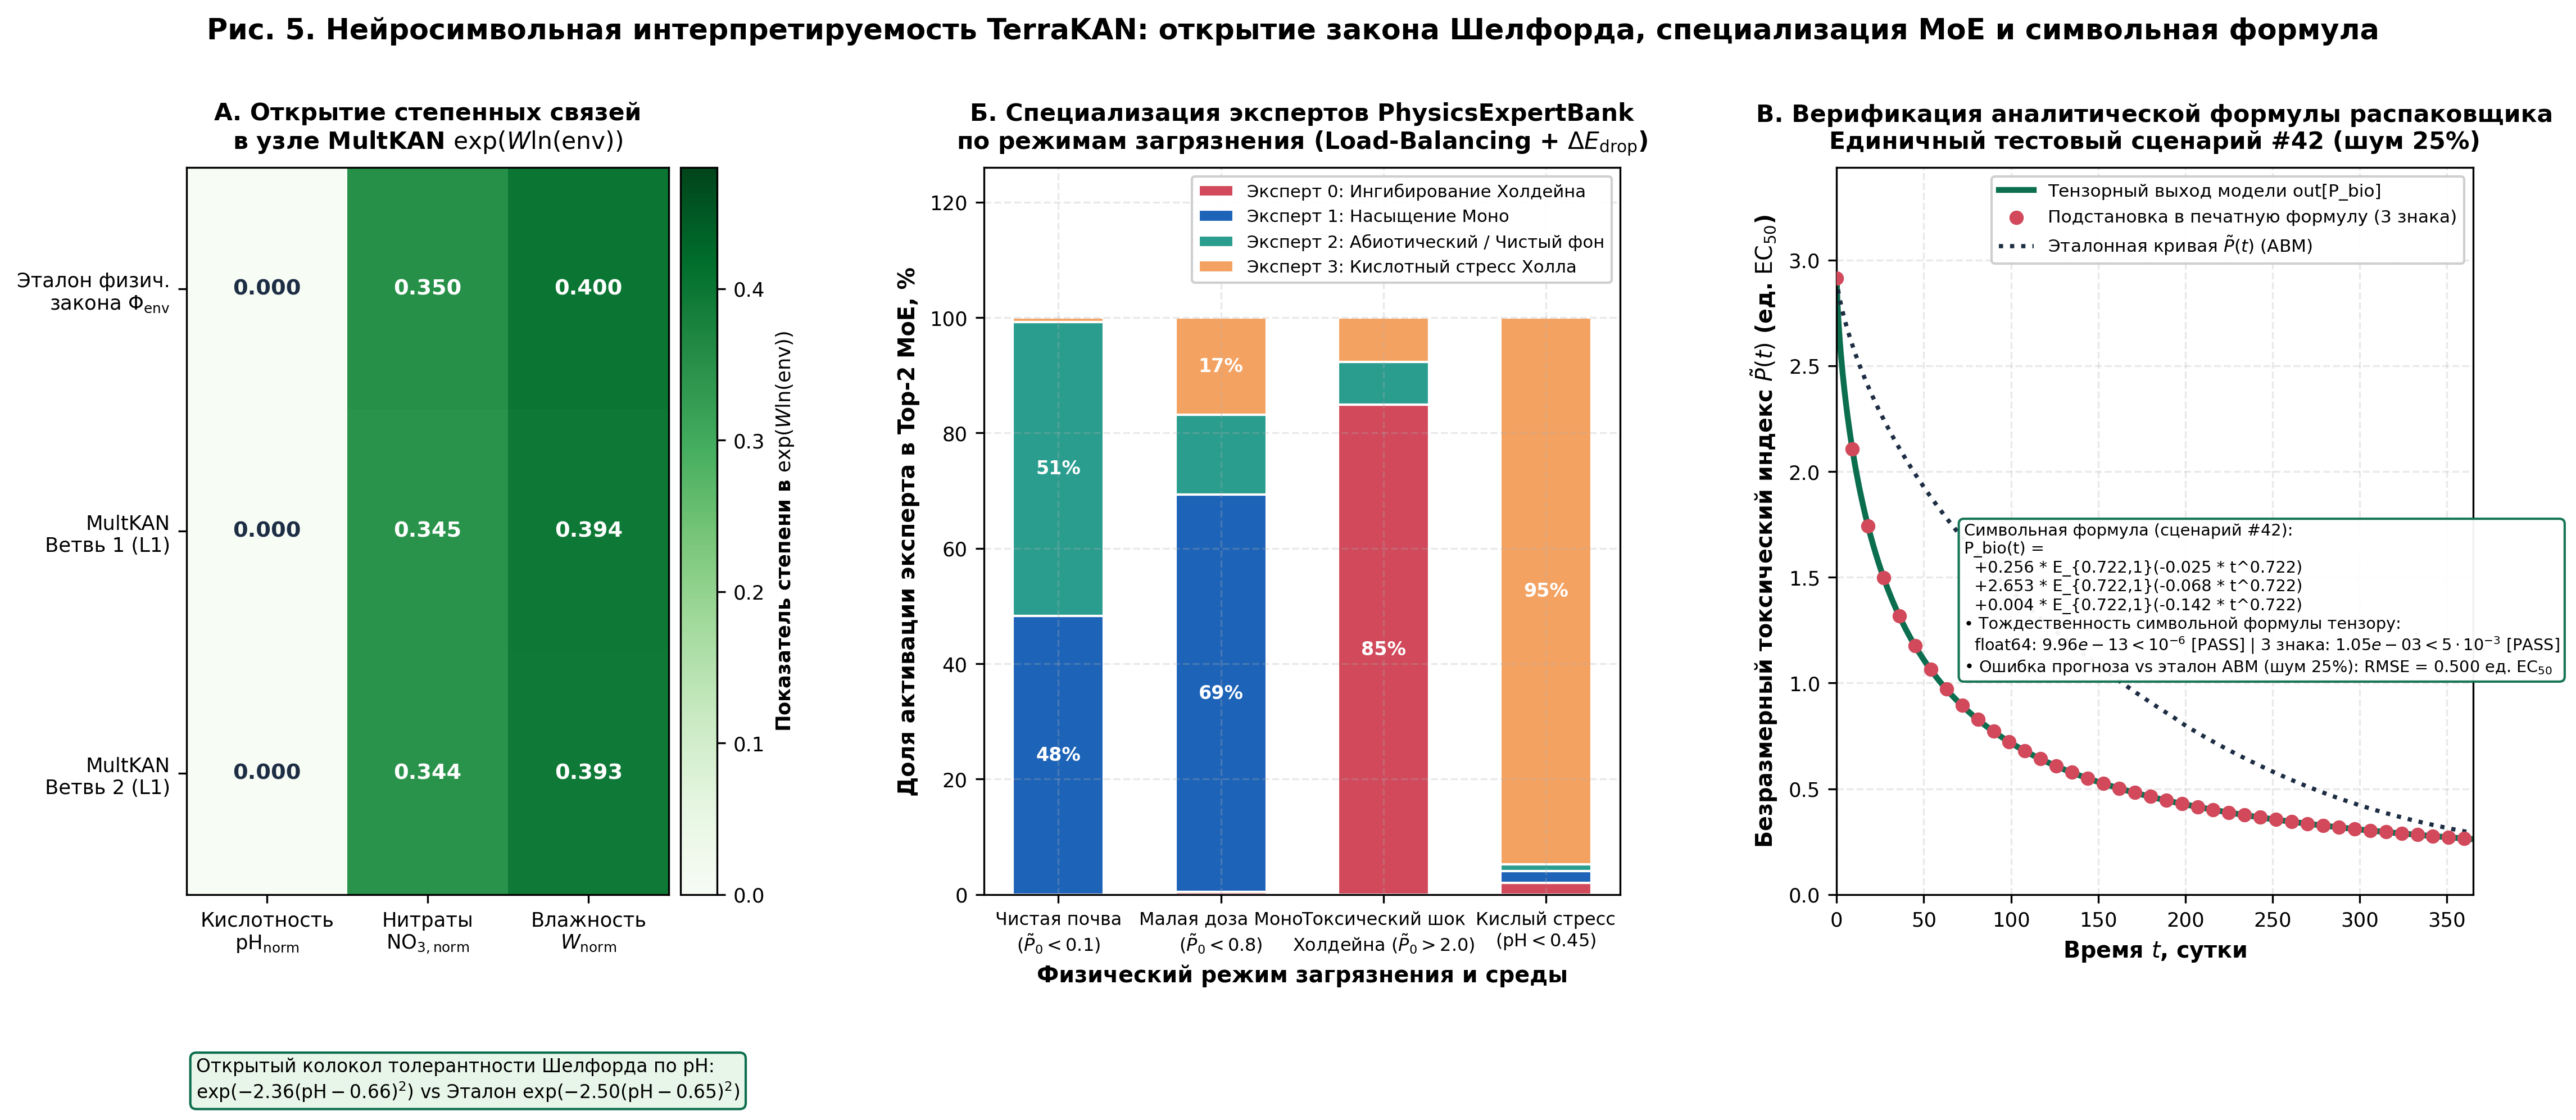
\includegraphics[width=0.95\textwidth]{fig5_multkan_symbolic_discovery.png}
  \vspace{-1mm}
  \caption{\textbf{Neuro-Symbolic Power-Law Discovery (\texttt{MultKAN}), Biokinetic MoE Routing, and Exact Symbolic Formula Audit.} \textbf{(A)} Recovery of nitrate ($0.345$) and moisture ($0.394$) exponents and Shelford pH bell. \textbf{(B)} Top-2 expert utilization across 4 regimes. \textbf{(C)} Exact identity between unpacked closed-form Mittag-Leffler strings and neural tensor output ($9.96\times 10^{-13}$ in \texttt{float64}).}
  \label{fig:fig5}
\end{figure*}

\begin{figure*}[!htbp]
  \centering
  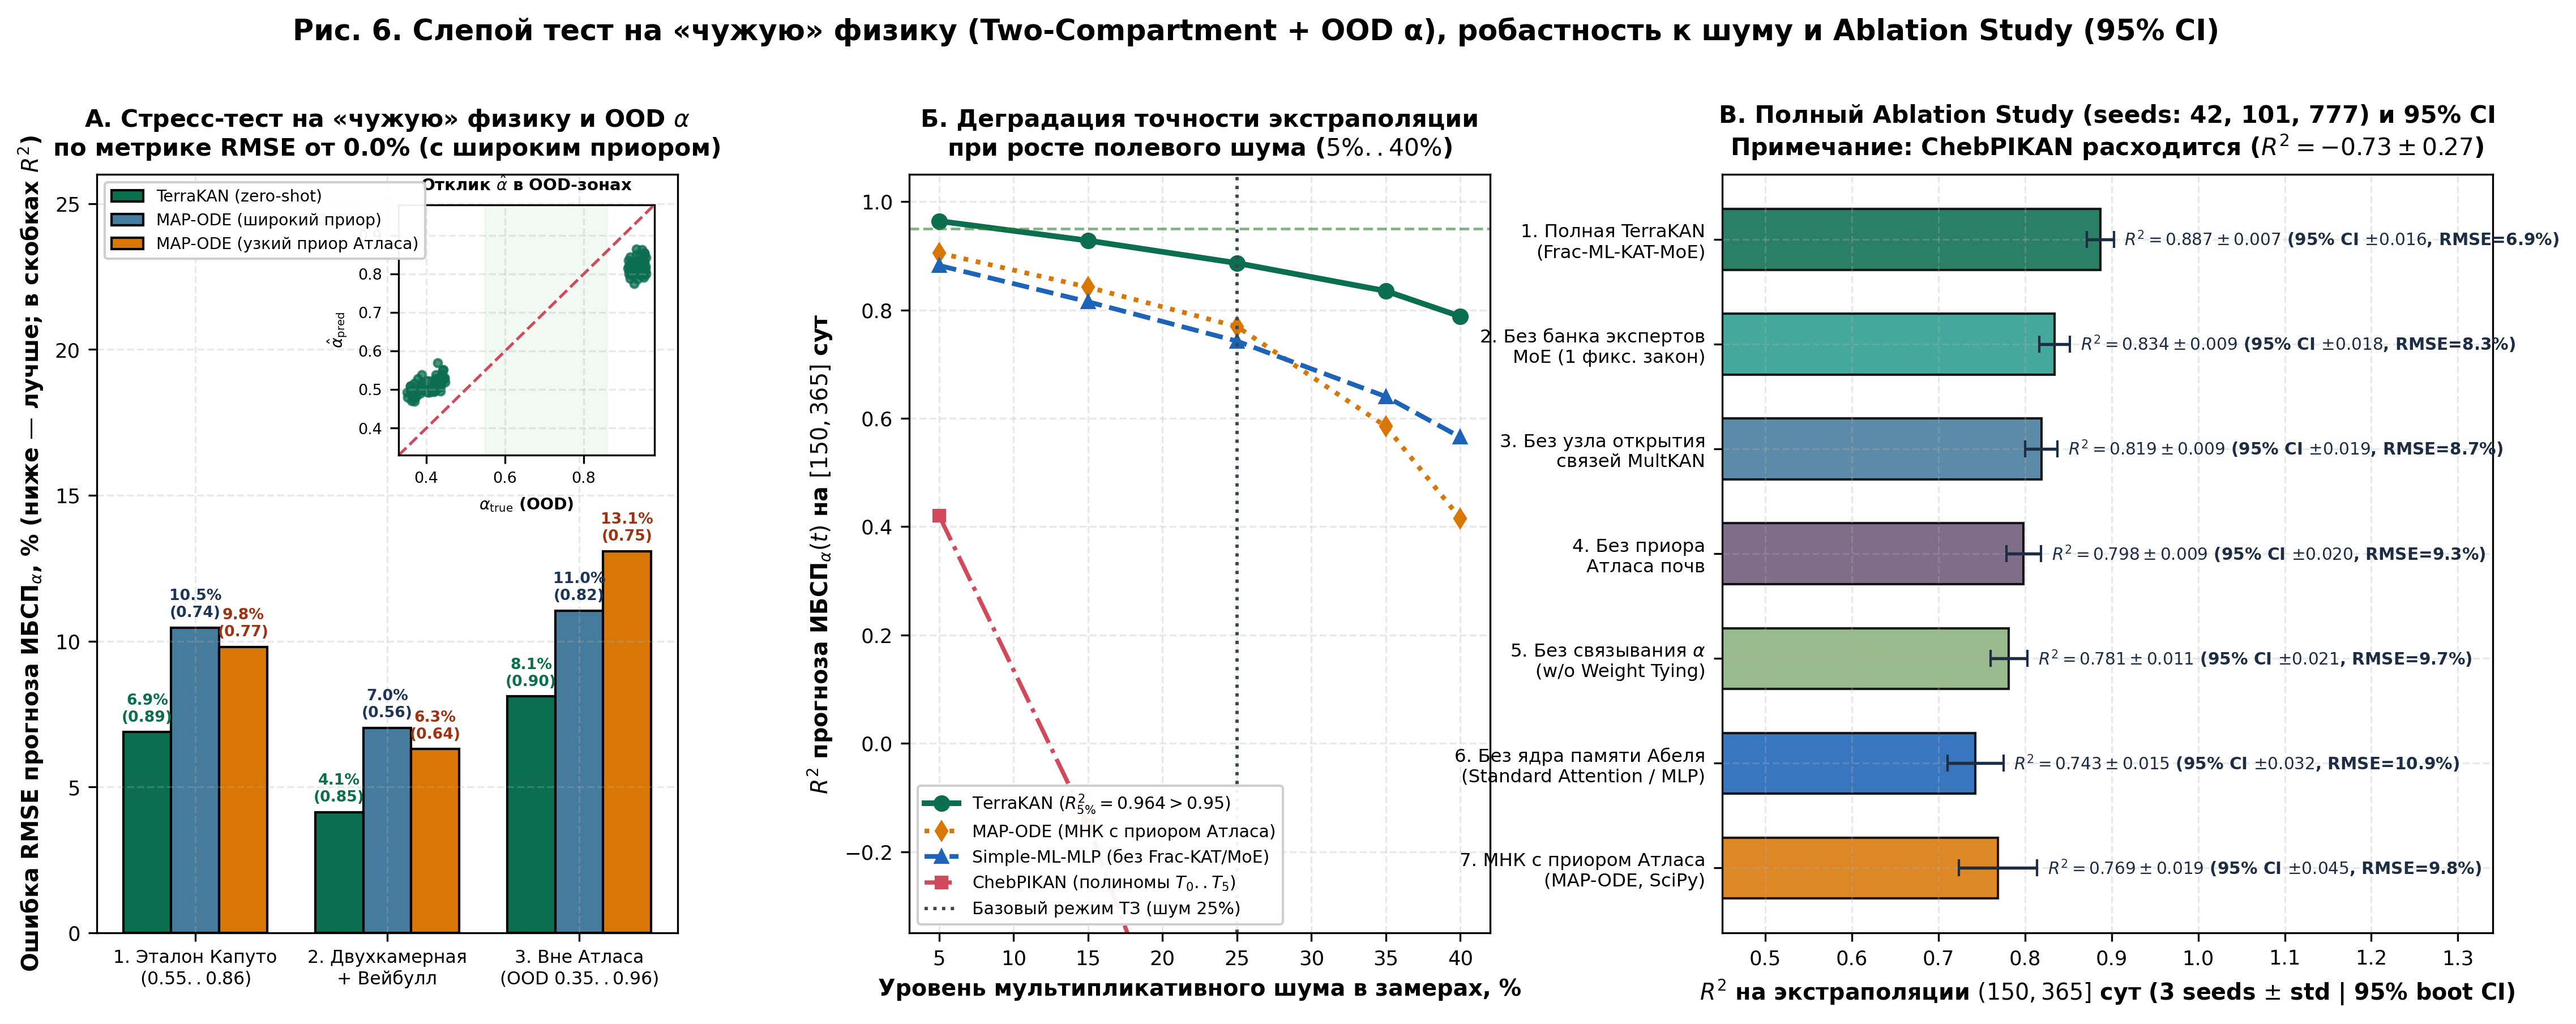
\includegraphics[width=0.95\textwidth]{fig6_ablation_and_noise_robustness.png}
  \vspace{-1mm}
  \caption{\textbf{Noise Robustness up to $40\%$, Zero-Shot Generalization to Alien Physics / OOD $\alpha$, and 3-Seed Ablation Study.}}
  \label{fig:fig6}
\end{figure*}

\begin{figure*}[!htbp]
  \centering
  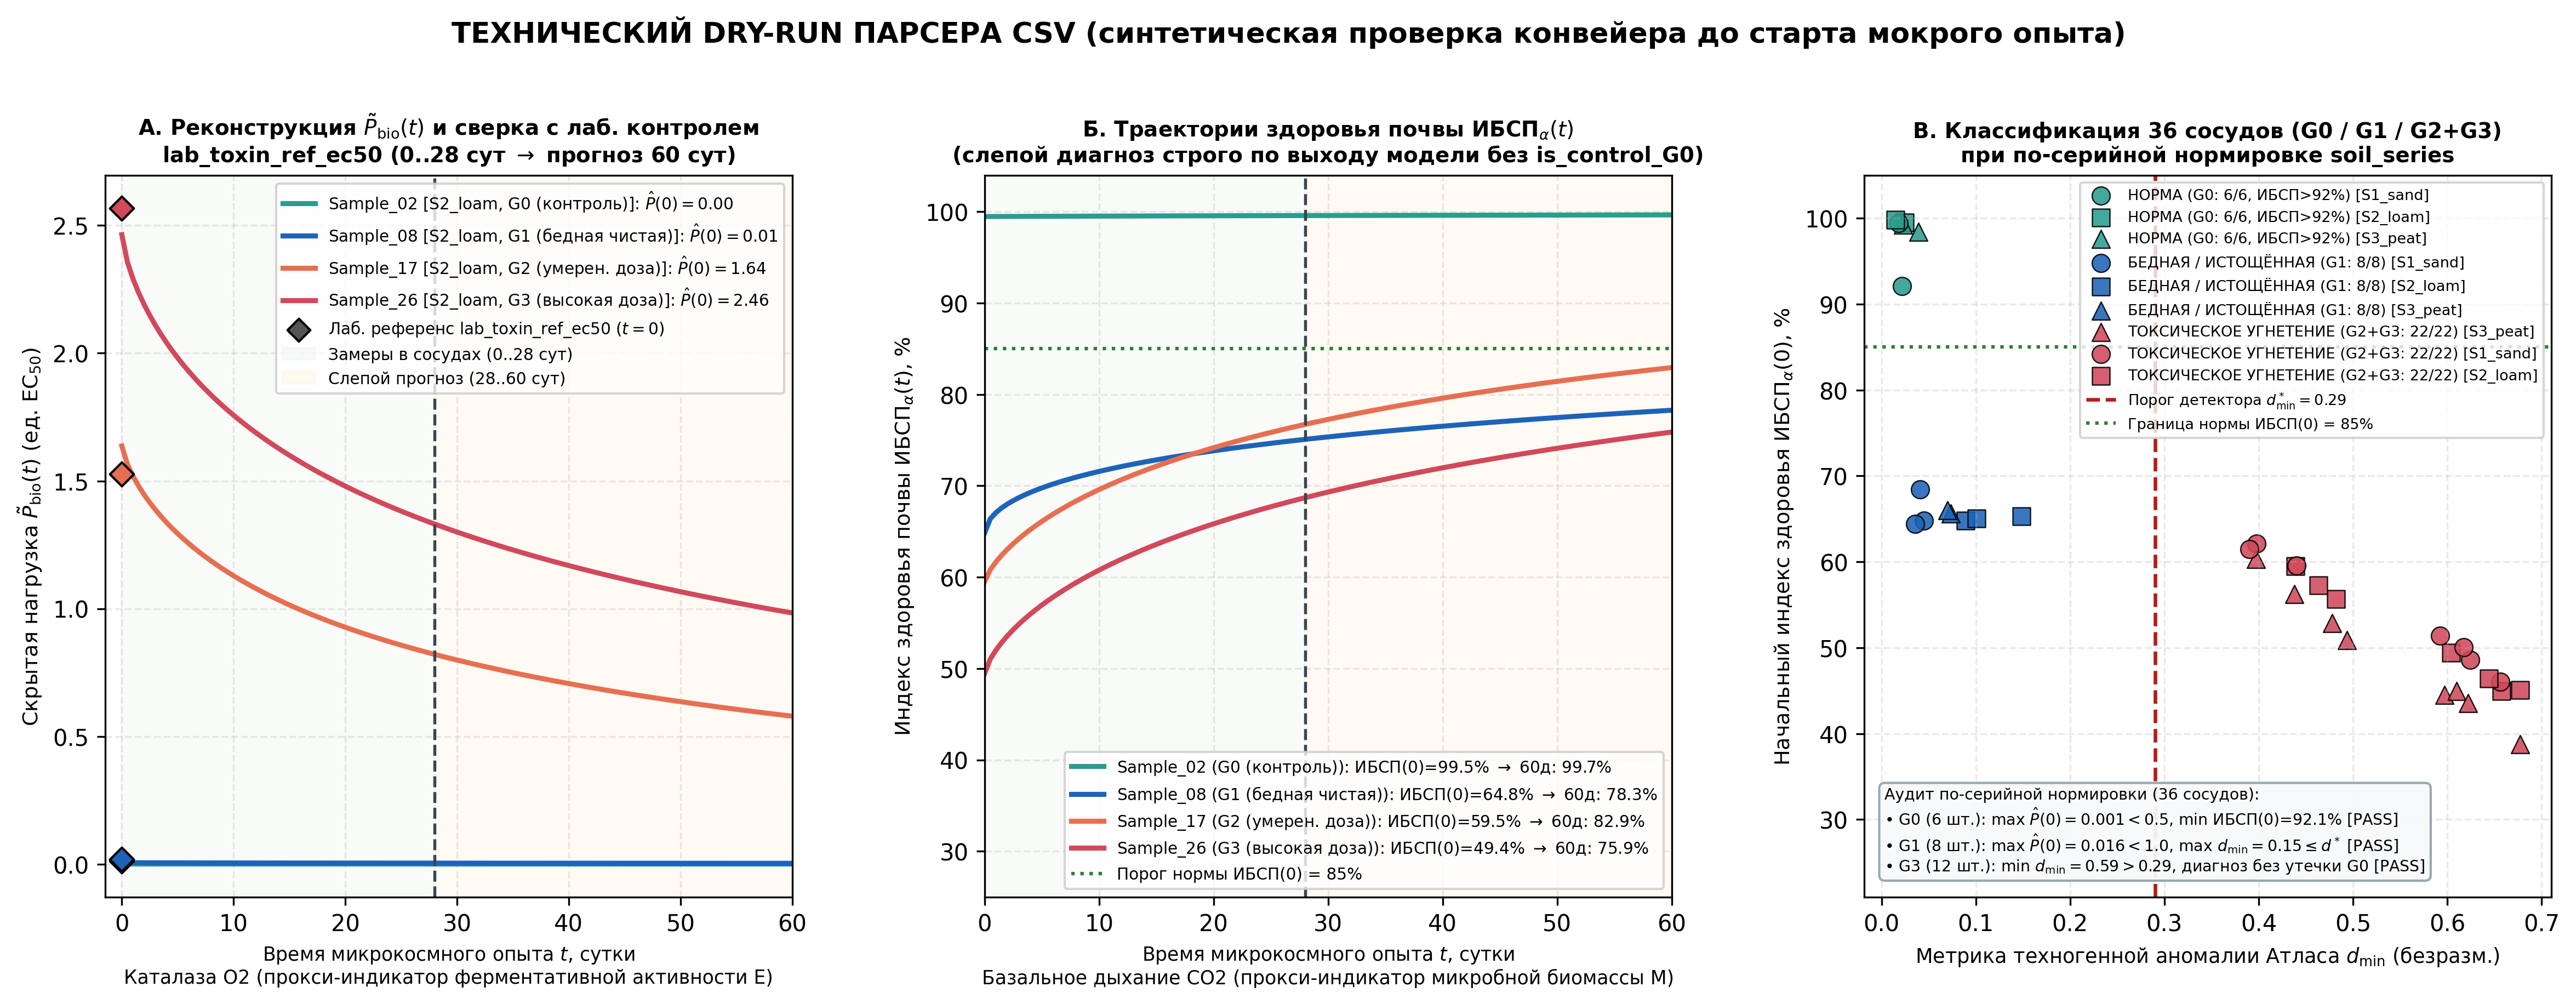
\includegraphics[width=0.95\textwidth]{fig_dry_run_36pots.png}
  \vspace{-1mm}
  \caption{\textbf{Technical Dry-Run Validation of Frozen Checkpoint \texttt{terrakan\_v4\_frozen.pt} on 36 Microcosm Vessels ($0\dots 28\text{ d} \to 60\text{ d}$).} Per-series control normalization (\texttt{S1\_sand}, \texttt{S2\_loam}, \texttt{S3\_peat}) and strictly model-driven diagnosis without \texttt{is\_control\_G0} leakage.}
  \label{fig:fig7}
\end{figure*}

\begin{thebibliography}{9}
\footnotesize
\setlength{\itemsep}{1.5pt}

\bibitem{tu2026fractional}
Tu, W., Liu, X., Wang, H., Li, X., \& Han, C. (2026). Fractional Calculus for Large Language Models: A Survey of Potentials, Mechanisms, and Challenges. \textit{Fractal and Fractional}, 10(7), 454. \href{https://doi.org/10.3390/fractalfract10070454}{https://doi.org/10.3390/fractalfract10070454}

\bibitem{liu2024kan}
Liu, Z., Wang, Y., Vaidya, S., et al. (2024). KAN: Kolmogorov-Arnold Networks. \textit{arXiv preprint} \href{https://arxiv.org/abs/2404.19756}{arXiv:2404.19756}.

\bibitem{liu2024kan2}
Liu, Z., Ma, P., Wang, Y., Matusik, W., \& Tegmark, M. (2024). KAN 2.0: Kolmogorov-Arnold Networks Meet Science (\texttt{MultKAN}). \textit{arXiv preprint} \href{https://arxiv.org/abs/2408.10205}{arXiv:2408.10205}.

\bibitem{yang2025kat}
Yang, X., \& Wang, X. (2025). Kolmogorov-Arnold Transformer. \textit{International Conference on Learning Representations (ICLR 2025)} / \href{https://arxiv.org/abs/2409.10594}{arXiv:2409.10594}.

\bibitem{aghaei2024rkan}
Aghaei, A. A. (2024). rKAN: Rational Kolmogorov-Arnold Networks. \textit{arXiv preprint} \href{https://arxiv.org/abs/2406.14495}{arXiv:2406.14495}.

\bibitem{aghaei2024fkan}
Aghaei, A. A. (2024). fKAN: Fractional Orthogonal Kolmogorov-Arnold Networks. \textit{arXiv preprint} \href{https://arxiv.org/abs/2406.07456}{arXiv:2406.07456}.

\bibitem{abueidda2025deepokan}
Abueidda, D. W., Pantidis, P., \& Mobasher, M. E. (2025). DeepOKAN: Deep Operator Network Based on Kolmogorov Arnold Networks for Mechanics Problems. \textit{Computer Methods in Applied Mechanics and Engineering}, 436, 117699. \href{https://doi.org/10.1016/j.cma.2024.117699}{https://doi.org/10.1016/j.cma.2024.117699}

\bibitem{yan2026soil}
Yan, C., et al. (2026). Soil carbon fractions rather than enzyme stoichiometry govern greenhouse gas reactivity to microplastics and metal oxides in hydrologically dynamic soils. \textit{Journal of Hazardous Materials}, 512, 142317.

\bibitem{diethelm2002predictor}
Diethelm, K., Ford, N. J., \& Freed, A. D. (2002). A predictor-corrector approach for the numerical solution of fractional differential equations. \textit{Nonlinear Dynamics}, 29, 3--22. \href{https://doi.org/10.1023/A:1016592219341}{https://doi.org/10.1023/A:1016592219341}

\bibitem{kazeev2016bio}
Kazeev, K. Sh., Kolesnikov, S. I., \& Valkov, V. F. (2003/2016). \textit{Biological Diagnostics and Indication of Soils: Methodology and Research Methods} [in Russian]. Rostov-on-Don: Southern Federal University Press.

\end{thebibliography}

\end{document}
